\documentclass[]{../template/Report}%方括号内写yuxi即生成预习报告\documentclass[yuxi]{../template/Report}
\settemplatedir{../template/}%设置模板路径

\exname{\small{用霍尔法测直流圆线圈与亥姆霍兹线圈磁场}} %实验名称
\extable{} %实验桌号
\instructor{} %指导教师
\class{} %班级
\name{} %姓名
\stuid{} %学号

\nyear{} %年
\nmonth{} %月
\nday{} %日
\nweekday{} %星期几,e.g. \nweekday{三}
\daypart{}%上午/下午,e.g. \daypart{上}

\redate{} %如有实验补做,补做日期
\resitu{} %情况说明:

\begin{document}
\makecover%输出封面
\section{预习报告(10分)}
\subsection{实验综述(5分)}
\subsubsection{载流圆线圈与亥姆霍兹线圈的磁场分布}
\textbf{载流圆线圈:}如下左图所示,半径为$R$,通以直流电流$I$的圆线圈,其轴线上离圆线圈中心距离为$X$米处的磁感应强度表达式为:
\[B = \frac{\mu_0 \cdot N_0 \cdot I \cdot R^2}{2 \cdot (R^2 + X^2)^{3/2}}\]为真空磁导率。磁场分布是一条单峰的关于线圈中心对称的曲线。

\vspace{2mm}
\textbf{亥姆霍兹线圈:}如下右图所示,两个完全相同的圆线圈彼此平行且共轴,通以同方向电流$I$,当线圈间距等于线圈半径$R$时,两线圈合磁场在中心轴线上(两线圈圆心连线)附近较大范围内是匀强磁场。
\begin{figure}[!h]
    \begin{center}
        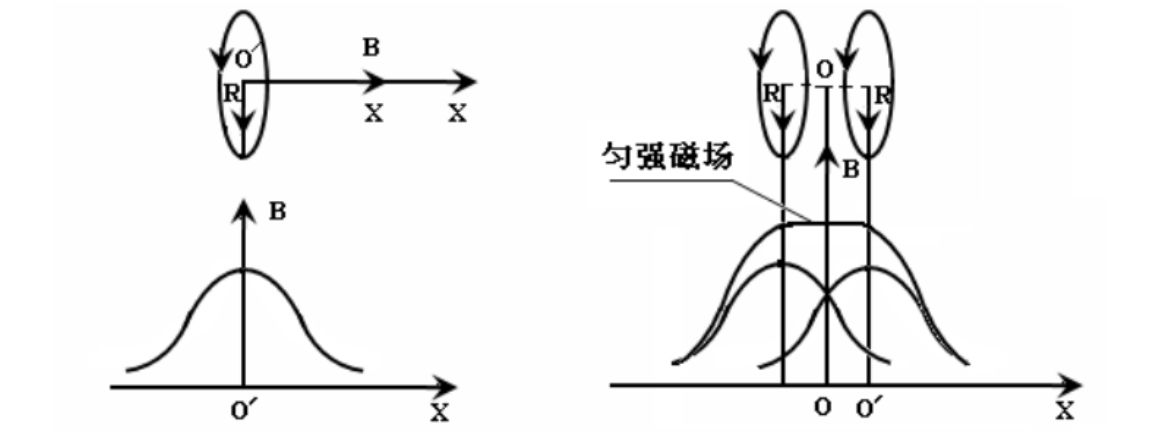
\includegraphics[width=0.7\textwidth]{figues/huoerfa/xianquan.png}
        \caption{载流圆线圈与亥姆霍兹线圈的磁场分布}
    \end{center}
\end{figure}
\vspace{-7mm}
\subsubsection{利用霍尔效应测磁场的原理}
霍尔元件的作用如下图所示,若电流$I$流过厚度为$d$的矩形半导体薄片,且磁场$B$垂直作用于该半导体,由于洛伦兹力作用电流方向会发生改变,在薄片两个横向面$a、b$之间产生的电势差称为霍尔电势\(U_H\)。霍尔电势差的产生是因为当电流\(I_H\)通过霍尔元件(假设为$P$型)时,空穴受洛伦兹力\(F_B = q \cdot (v \times B)\)产生横向偏转,在边界积累形成横向电场$E$,直到电场力\(F_E = q \cdot E\)与洛伦兹力相抵消,此时霍尔电势差由该电场建立。
\begin{figure}[!h]
    \begin{center}
        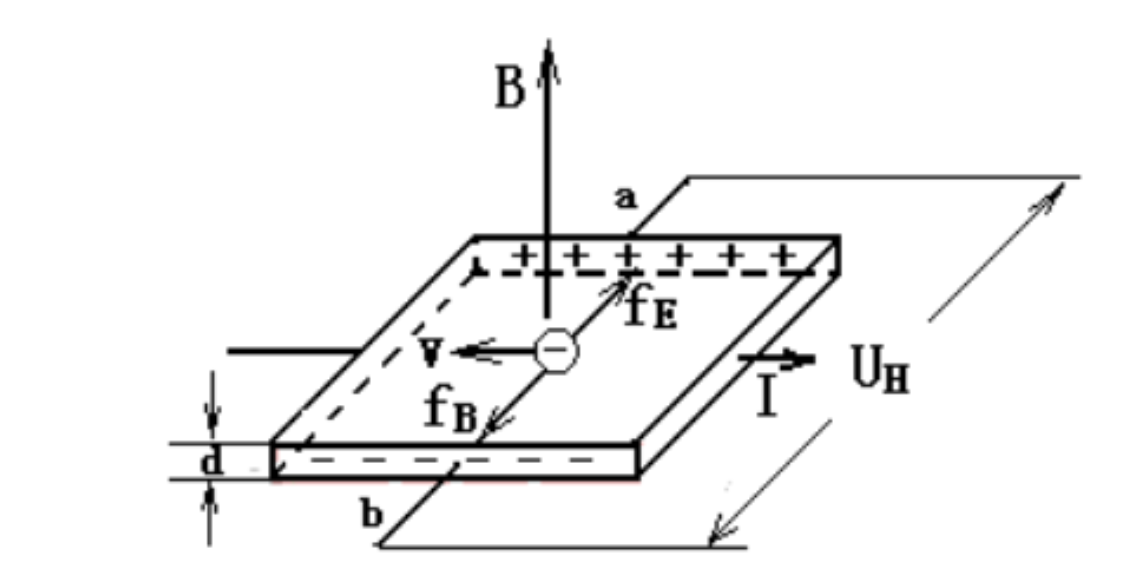
\includegraphics[width=0.5\textwidth]{figues/huoerfa/huoerxiaoying.png}
        \caption{利用霍尔效应测磁场的原理}
    \end{center}
\end{figure}

霍尔电势\(U_H\)的表达式为:
\[U_H = K_H \cdot I_H \cdot B\]
其中比例系数\(K_H\)称为霍尔元件的灵敏度,单位为\(\text{mV/(mA·T)}\)。只要分别测出霍尔电流\(I_H\)及霍尔电势差\(U_H\)就可以算出磁场$B$的大小,这就是霍尔效应测量磁场的原理。
\subsubsection{实验方法}
\begin{enumerate}
    \item 测量载流圆线圈轴线上磁场的分布;
    \item 测量亥姆霍兹线圈轴线上磁场的分布;
    \item 测量载流圆线圈沿径向的磁场分布;
    \item 改变线圈间距。
\end{enumerate}
\subsubsection{实验现象}
\begin{enumerate}
    \item 测量载流圆线圈轴线上磁场分布时,随着测试点与线圈中心距离$X$的变化,磁感应强度$B$呈现出单峰且关于线圈中心对称的变化规律,中心处磁感应强度最大,向两侧逐渐减小。
    \item 测量亥姆霍兹线圈轴线上磁场分布时,在两线圈中心连线一段会出现磁感应强度基本不变的平台区域,呈现出匀强磁场的特征,在该区域外,磁感应强度逐渐减小。
    \item 测量载流圆线圈沿径向的磁场分布时,随着径向距离$Y$的变化,磁感应强度$B$也会发生相应变化。
    \item 改变亥姆霍兹线圈间距为\(d = R/2\)和\(d = 2R\)时,轴线上的磁场分布规律与间距为\(d = R\)时不同,平台区域的长度和磁感应强度大小等都会发生改变。
\end{enumerate}

\subsection{实验重点(3分)}
\begin{enumerate}
    \item 了解用霍尔效应法测量磁场的原理,掌握FB511型霍尔法亥姆霍兹线圈磁场实验仪的使用方法;
    \item 了解载流圆线圈的径向磁场分布情况;
    \item 测量载流圆线圈和亥姆霍兹线圈的轴线上的磁场分布;
    \item 两平行线圈的间距改变为\(d = R / 2\)和\(d = 2R\)时,测定其轴线上的磁场分布。
\end{enumerate}
\subsection{实验难点(2分)}
\begin{enumerate}
    \item 精准操作实验仪器,如稳定调节励磁电流、准确移动传感器探头;
    \item 把控霍尔元件特性,依据其参数准确计算磁场;
    \item 有效消除地磁场、杂散干扰及不平衡电势等系统误差。
\end{enumerate}
\clearpage
\begin{fullreportonly}
\section{原始数据(20分)}
\begin{figure}[!h]
    \begin{center}
        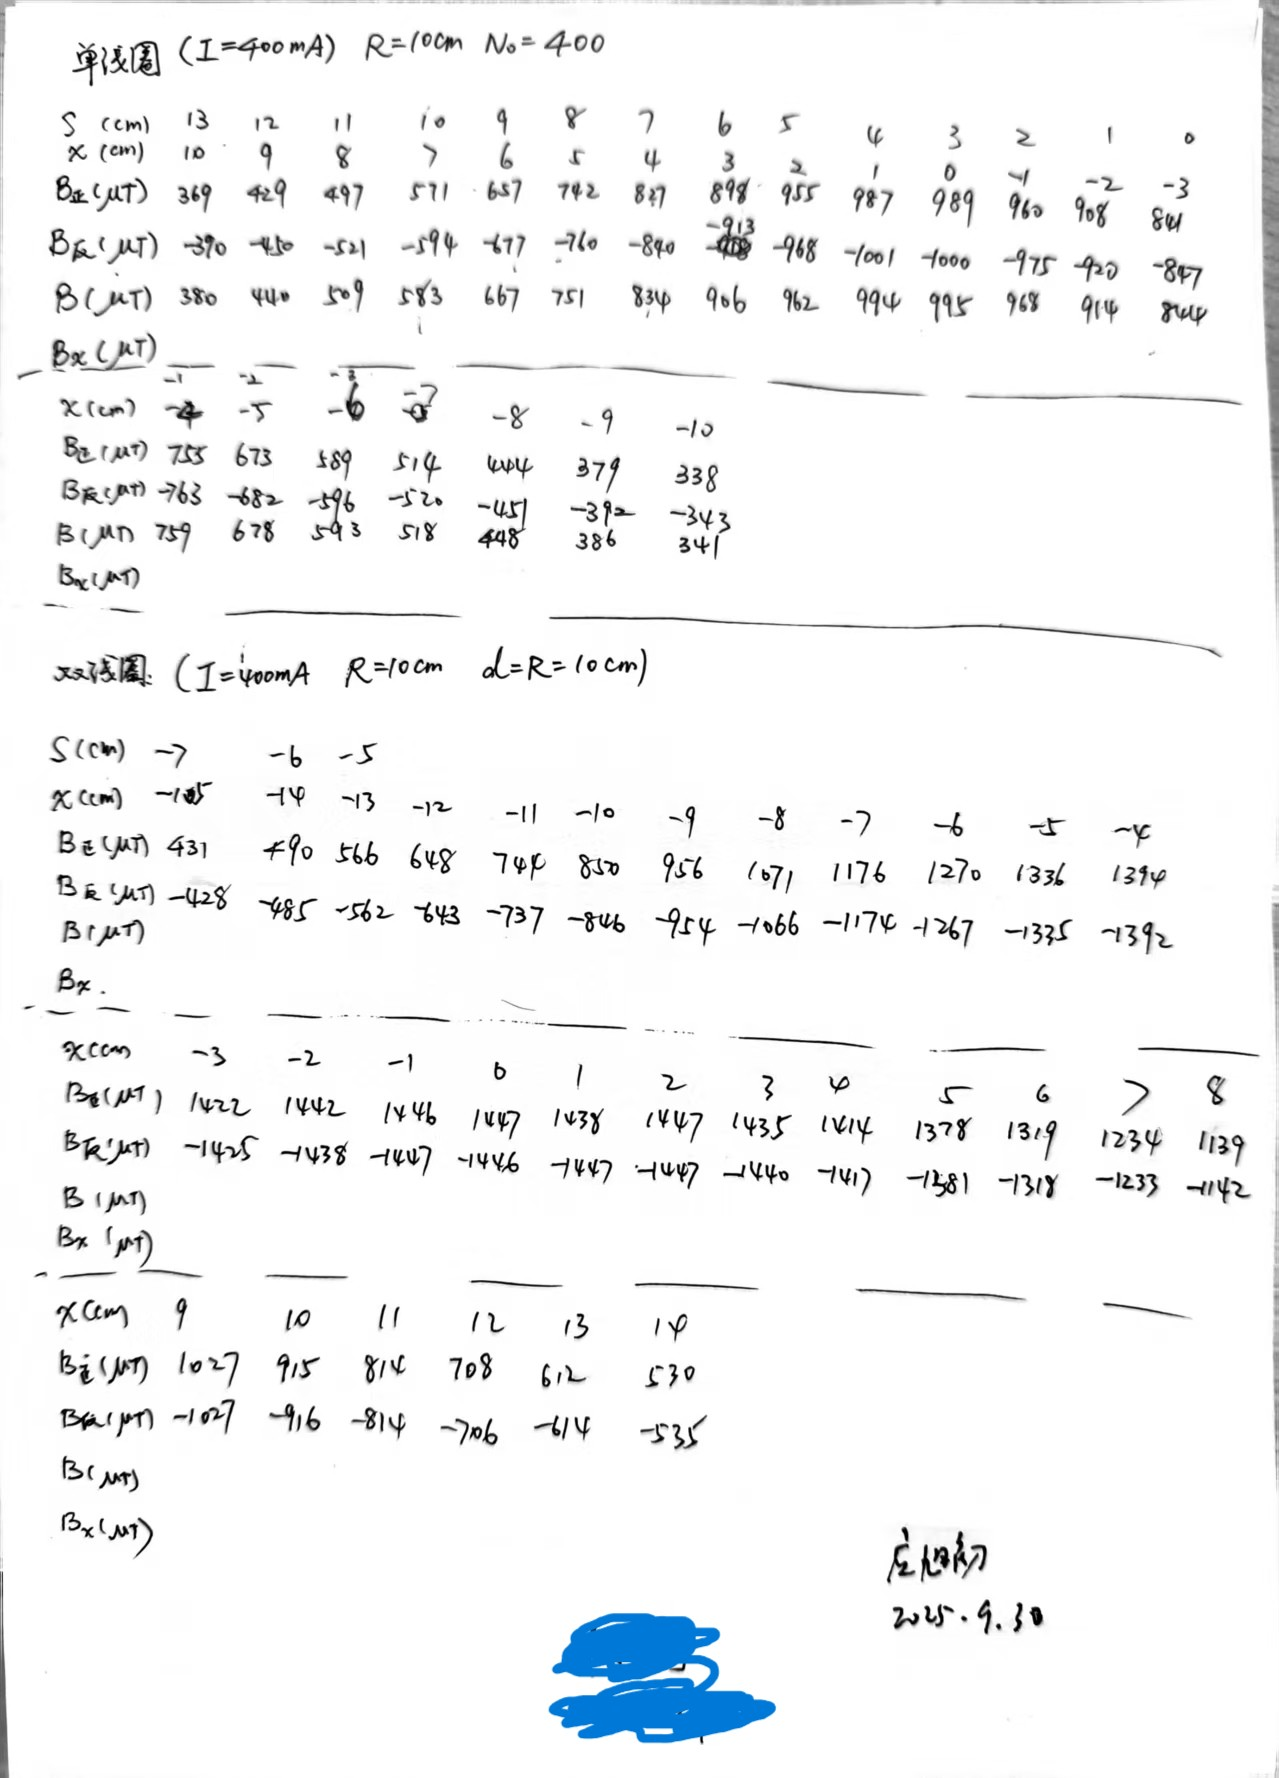
\includegraphics[width=0.7\textwidth]{exp_data/huoerfa.jpg}
        \caption{原始数据}
    \end{center}
\end{figure}
\section{结果与分析(60分)}
\subsection{数据处理与结果(30分)}
\subsubsection{测量地磁场}
实验中,先测量地磁场,将仪器东西向放置,调零,最后南北向放置,记录地磁场数据如下表:
\begin{table}[htbp]
  \centering
  \caption{地磁场强度测量数据}
  \begin{tabular}{ccccccc}
    \toprule
    序号 & 1 & 2 & 3 & 4 & 5 & 6 \\
    \midrule
    $B$ ($\mu\text{T}$)   & 22 & 21 & 22 & 21 & 22 & 21 \\
    \bottomrule
  \end{tabular}
\end{table}

\textbf{计算平均值:}平均值$\bar{B} = \frac{1}{n} \sum_{i=1}^n B_i= \frac{129}{6} = 21.5 \, \mu\text{T}$

\vspace{2mm}
\textbf{计算A类不确定度:}代入公式:
\[
s_{\bar{B}} = \sqrt{\frac{1}{n(n-1)} \sum_{i=1}^n (B_i - \bar{B})^2}
\]
得$s \approx 0.55 \, \mu\text{T}$
\subsubsection{测绘单个圆线圈磁场强度分布}
实验中,将线圈置于$S=13cm$处,给线圈通上电流,将霍尔传感器放置在距线圈轴线中心的不同距离,测得正向磁场强度与反向磁场强度,再根据公式
\[B = \frac{\mu_0 N_0  I  R^2}{2  (R^2 + X^2)^{3/2}}\]
代入$I=400mA,N_0=400,R=10cm,\mu_0 = 4\pi \times 10^{-7}$得到不同距离下的理论磁场强度$B_x$,数据如下:
\begin{table}[h]
    \centering
    \caption{单线圈磁场实验与理论数据(\( I = 400\,\text{mA} \),\( R = 10\,\text{cm} \),\( N_0 = 400 \))}
    \begin{tabular}{c c c c c c c c c c c c}
        \toprule
        $距离x(cm)$ & 10 & 9 & 8 & 7 & 6 & 5 & 4 & 3 & 2 & 1 & 0 \\
        \midrule
        \( B_{\text{正}} \, (\mu\text{T}) \) & 369 & 429 & 497 & 571 & 657 & 742 & 837 & 898 & 955 & 987 & 989 \\
        \( B_{\text{反}} \, (\mu\text{T}) \) & -390 & -450 & -521 & -594 & -677 & -760 & -840 & -913 & -968 & -1001 & -1000 \\
        \( B \, (\mu\text{T}) \) & 380 & 440 & 509 & 583 & 667 & 751 & 834 & 906 & 962 & 994 & 995 \\
        \( B_{\text{理}} \, (\mu\text{T}) \) & 355 & 413 & 479 & 553 & 634 & 719 & 805 & 883 & 948 & 990 & 1005 \\
        \bottomrule
    \end{tabular}
    \label{tab:magnetic-field-1}
\end{table}
\begin{table}[h]
    \centering
    \begin{tabular}{c c c c c c c c c c c}
        \toprule
       $ 距离x(cm) $& -1 & -2 & -3 & -4 & -5 & -6 & -7 & -8 & -9 & -10 \\
        \midrule
        \( B_{\text{正}} \, (\mu\text{T}) \) & 960 & 908 & 841 & 755 & 673 & 589 & 514 & 444 & 379 & 338 \\
        \( B_{\text{反}} \, (\mu\text{T}) \) & -975 & -920 & -847 & -763 & -682 & -596 & -520 & -457 & -392 & -343 \\
        \( B \, (\mu\text{T}) \) & 968 & 914 & 844 & 759 & 678 & 593 & 518 & 448 & 386 & 341 \\
        \( B_{\text{理}} \, (\mu\text{T}) \) & 990 & 948 & 883 & 805 & 719 & 634 & 553 & 479 & 413 & 355 \\
        \bottomrule
    \end{tabular}
\end{table}
\clearpage
绘制出载流圆单线圈轴线上的磁场分布如下图:
\begin{figure}[!h]
    \begin{center}
        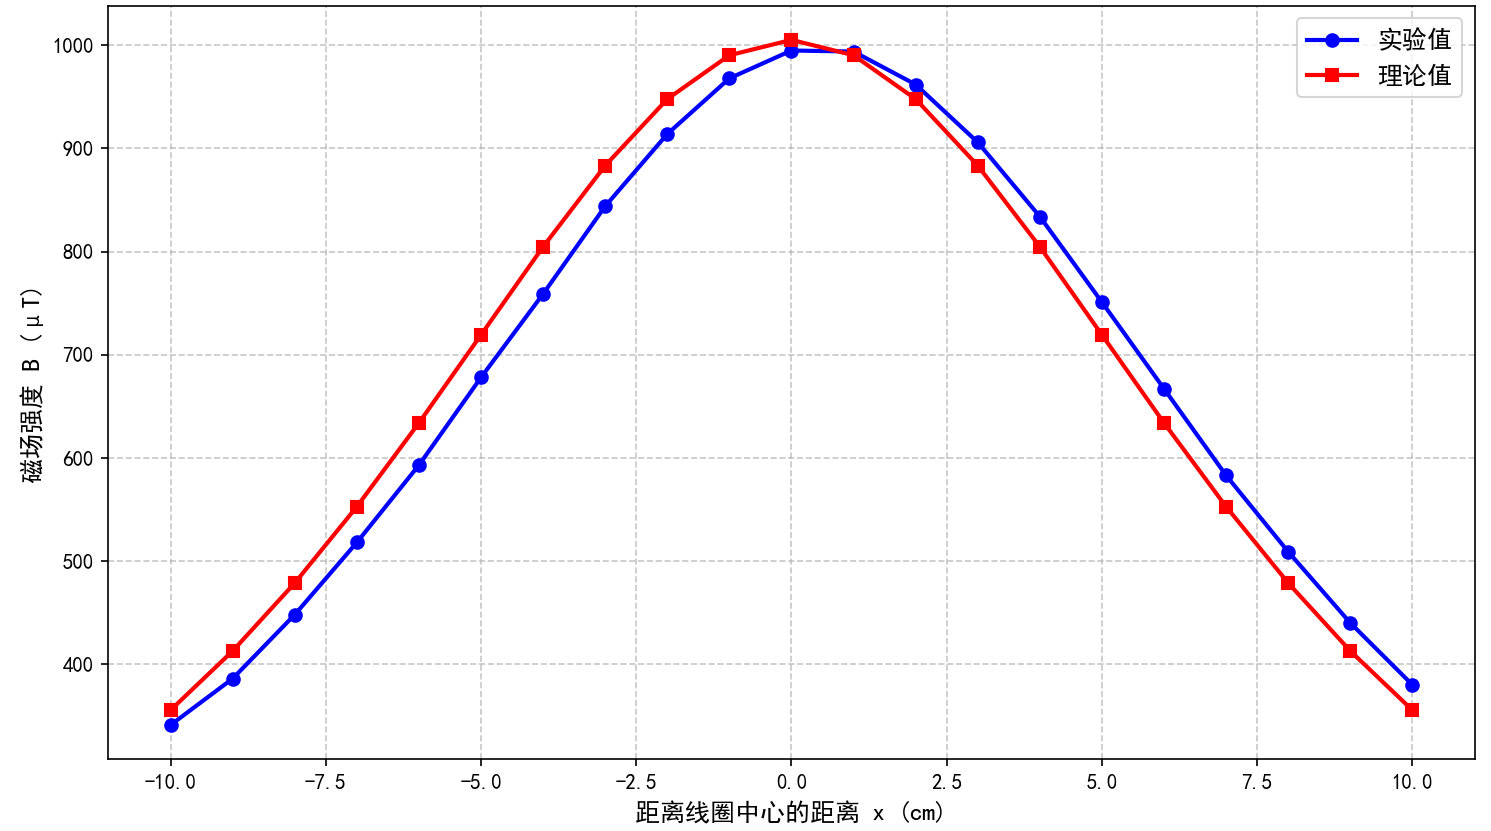
\includegraphics[width=0.7\textwidth]{figues/huoerfa/dxqquxian}
        \caption{载流圆单线圈轴线上的磁场分布}
    \end{center}
\end{figure}

\textbf{分析曲线特性:}磁场分布是一条单峰的关于线圈中心对称的曲线。

\vspace{2mm}
\textbf{计算圆心$B-B_x$相对误差:}$\text{相对误差} = \left| \frac{995  - 1005}{1005 } \right| \times 100\%\approx 1.0\%$
\subsubsection{测绘亥姆霍兹线圈磁场强度分布}
实验中,将两线圈分别放置在$10cm$与$20cm$处,将两线圈串联并通上电流,测得不同距离下的磁场强度,数据如下:
\begin{table}[h]
    \centering
    \caption{双线圈磁场实验数据}
    \begin{tabular}{c c c c c c c c c c c c}
        \toprule
      $距离x(cm)$ & 0 & 1 & 2 & 3 & 4 & 5 & 6 & 7 & 8 & 9 & 10 \\
        \midrule
        \( B_{\text{正}} \, (\mu\text{T}) \) & 1447 & 1438 & 1447 & 1435 & 1445 & 1328 & 1309 & 1234 & 1139 & 1027 & 915 \\
        \( B_{\text{反}} \, (\mu\text{T}) \) & -1446 & -1447 & -1447 & -1440 & -1441 & -1381 & -1328 & -1233 & -1142 & -1027 & -916 \\
        \( B \, (\mu\text{T}) \) & 1447 & 1443 & 1447 & 1438 & 1443 & 1355 & 1319 & 1234 & 1141 & 1027 & 916 \\
        \bottomrule
    \end{tabular}
\end{table}
\begin{table}[h]
    \centering
    \begin{tabular}{c c c c c c c c c c c c}
        \toprule
      $ 距离x(cm)$ & -1 & -2 & -3 & -4 & -5 & -6 & -7 & -8 & -9 & -10 \\
        \midrule
        \( B_{\text{正}} \, (\mu\text{T}) \) & 1446 & 1442 & 1422 & 1396 & 1336 & 1270 & 1176 & 1071 & 956 & 830 \\
        \( B_{\text{反}} \, (\mu\text{T}) \) & -1447 & -1438 & -1425 & -1392 & -1335 & -1267 & -1174 & -1066 & -954 & -846 \\
        \( B \, (\mu\text{T}) \) & 1447 & 1440 & 1424 & 1394 & 1336 & 1269 & 1175 & 1069 & 955 & 838 \\
        \bottomrule
    \end{tabular}
\end{table}

\clearpage
绘制出亥姆霍兹线圈磁场强度分布如下图:
\begin{figure}[!h]
    \begin{center}
        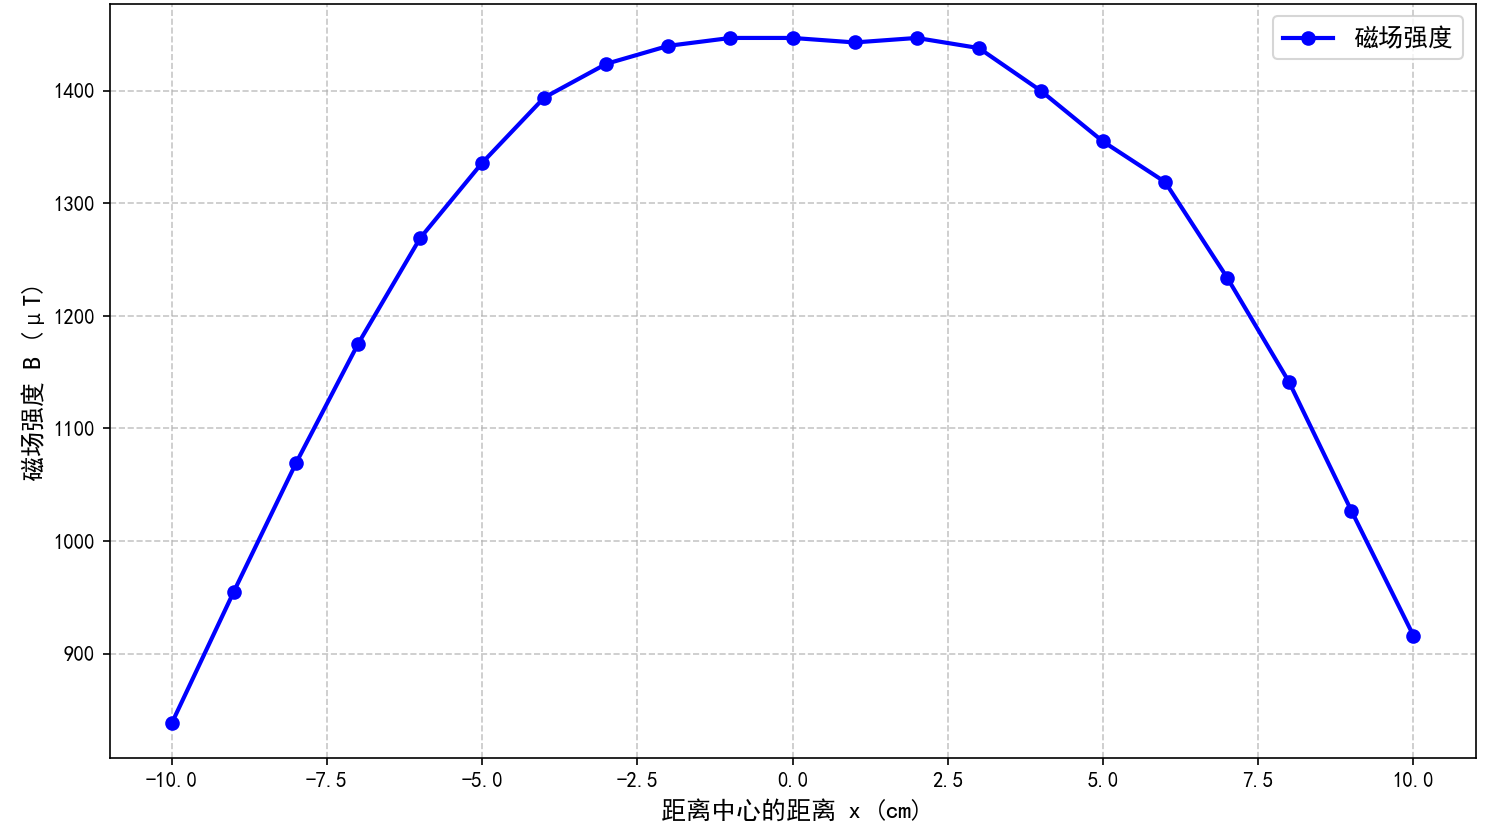
\includegraphics[width=0.7\textwidth]{figues/huoerfa/sxqqx.png}
        \caption{亥姆霍兹线圈磁场强度分布}
    \end{center}
\end{figure}

\textbf{分析曲线特性:}在两线圈中心连线一段,出现一个平台,说明此处为匀强磁场。
\subsection{误差分析(20分)}
\begin{enumerate}
    \item 实验中用于测量磁场的霍尔元件,其灵敏度并非绝对恒定,且实际的霍尔电压与磁场强度的关系可能存在一定的非线性偏差;
    \item 即使在无磁场的环境下,测量仪器也可能存在微小的输出电压;
    \item 实验过程中,若实验平台存在微小的振动或者位移,会使霍尔元件与线圈的相对位置发生变化,从而导致测量的磁场强度不是对应位置的真实值,产生系统误差。
    \item 实验环境中可能存在其他的电磁设备,它们产生的杂散磁场会叠加到双线圈产生的磁场之上,使测量到的磁场强度包含干扰信号,从而产生随机误差。
\end{enumerate}

\subsection{实验探讨(10分)}
\begin{enumerate}
    \item 通过测量载流线圈轴线上和径向的磁场分布,我直观地验证了理论公式的准确性;
    \item 数据记录与处理过程中,学会了如何合理选择测量点、如何通过多次测量减小随机误差;
    \item 掌握了用 Python 等工具将实验数据可视化的方法。
\end{enumerate}

\section{思考题(10分)}
\subsection{为什么在测量直流磁场时,必须考虑地球磁场对被测磁场的影响。}
地球磁场会叠加到被测直流磁场,若被测磁场与地磁场量级相当,会显著影响测量结果。
\subsection{载流圆线圈轴线上磁场的分布规律如何?}
载流圆线圈轴线上磁场,中心处最强,向两端逐渐减弱,且关于中心对称。
\subsection{亥姆霍兹线圈是怎样组成的?其基本条件有哪些?它的磁场分布特点又怎样?改变两圆线圈间距后,线圈轴线上的磁场分布情况如何?}
亥姆霍兹线圈由两个相同载流圆线圈平行共轴组成,基本条件是间距等于线圈半径;轴线上中间区域磁场均匀性好。改变间距后,均匀磁场区域会改变,间距偏离半径时均匀性变差。
\subsection{霍尔元件放入磁场时,不同方向上特斯拉计指示值不同,哪个方向最大?}
霍尔元件平面垂直于磁场方向时,特斯拉计指示值最大。
\subsection{试分析载流圆线圈磁场分布的理论值与实验值的误差产生的原因?}误差源于仪器精度、环境干扰(如地磁场、杂散磁场)、线圈绕制精度、测量操作等。
\end{fullreportonly}
\insertnotes
\end{document}
